\documentclass[11pt]{article}
\usepackage[margin=1in]{geometry}
\usepackage{amsmath,amssymb,amsthm,booktabs,graphicx}
\usepackage[colorlinks=true,linkcolor=blue,urlcolor=blue]{hyperref}
\special{pdf:minorversion 7}
\newtheorem{theorem}{Theorem}
\newtheorem{lemma}[theorem]{Lemma}
\newtheorem{corollary}[theorem]{Corollary}
\newcommand{\F}{\mathbf F}
\newcommand{\Z}{\mathbf Z}
\newcommand{\OK}{\mathcal O_M}
\newcommand{\Nm}{\operatorname{N}}
\newcommand{\End}{\operatorname{End}}
\title{A norm-one conductor obstruction\protect\\for weak elliptic curves}
\author{ISO-1 research note}
\date{October 8, 2026}
\begin{document}
\maketitle
\begin{abstract}
For an odd extension of a finite field of size $q\equiv1\pmod4$, a
Legendre parameter in the norm-one subgroup is a fourth power. Its
rational $2$-isogeny has a target with full rational $4$-torsion. Thus
one quadratic-twist sign has cardinality divisible by $16$; in an
ordinary isogeny class, this is equivalent to $4$ dividing the
Frobenius-order conductor. This proves the depth-one exclusion in the
$q=p^2$, cubic-extension census at every odd prime, independently of
the computed labels. We also prove that absolute Frobenius and inversion
reduce that census to exactly $(p^4+3p^2+8)/12$ point-count calls for
$p>3$, with explicit exceptional-orbit weights.
\end{abstract}

\section{The norm-one obstruction}
Let $k=\F_q$, let $n\ge3$ be odd, and put $K=\F_{q^n}$ and $Q=q^n$.
Assume $q$ is odd and $q\equiv1\pmod4$. Write $\sigma(z)=z^q$ and
\[
 T=\ker(\Nm_{K/k}:K^\times\longrightarrow k^\times),
 \qquad N=|T|=1+q+\cdots+q^{n-1}.
\]
The generalized weak family is
\[
 E_\alpha:\quad y^2=x(x-\alpha)(x-\sigma\alpha),
 \qquad \alpha\in K\setminus k.
\]
This is the cubic weak model used in the census when $q=p^2$ and $n=3$.
An affine root translation or a quadratic twist preserves the conclusion
below whenever the resulting Legendre parameter belongs to $T$.

\begin{theorem}[Norm-one conductor obstruction]\label{thm:main}
For every $\alpha\in K\setminus k$, put
$\lambda=\sigma(\alpha)/\alpha$. Then $\lambda\in T\setminus\{1\}$,
and the Legendre curve
\[
 L_\lambda:\quad y^2=x(x-1)(x-\lambda)
\]
has a rational $2$-isogeny whose target has full rational $4$-torsion.
If $t=Q+1-\#E_\alpha(K)$, then
\begin{equation}\label{eq:trace}
 t\equiv\pm(Q+1)\pmod{16}.
\end{equation}
If $E_\alpha$ is ordinary, write
\[
 t^2-4Q=f_\pi^2D_M,
\]
where $D_M$ is the fundamental discriminant of its imaginary quadratic
endomorphism algebra and $f_\pi=[\OK:\Z[\pi]]$. Then
\begin{equation}\label{eq:conductor}
 4\mid f_\pi,\qquad v_2(f_\pi)\ge2.
\end{equation}
\end{theorem}

\begin{proof}
The norm of $\lambda$ telescopes to $1$. The integer $N$ is odd, so
raising to the fourth power is an automorphism of the cyclic group $T$.
Choose $\mu\in T$ with $\lambda=\mu^4$ and put $s=\mu^2$.
For $n=3$ one can take
\[
 \mu=\lambda^{(q^2+q+2)/4}.
\]
Here $\lambda\ne0,1$, since $\alpha\ne0$ and $\sigma\alpha\ne\alpha$.

Set $a=-(1+\lambda)$ and $b=\lambda$. On
$L_\lambda:y^2=x^3+ax^2+bx$, the map
\begin{equation}\label{eq:map}
 (x,y)\longmapsto
 \left(x+a+\frac b x,\ y\left(1-\frac b{x^2}\right)\right)
\end{equation}
for $x\ne0$, with $O$ and $(0,0)$ mapped to $O$, is the rational
$2$-isogeny with kernel $\{O,(0,0)\}$. Its target is
\begin{align*}
 L'_\lambda:\quad y^2
 &=x\bigl(x^2-2ax+(a^2-4b)\bigr)\\
 &=x\bigl(x+(1+s)^2\bigr)\bigl(x+(1-s)^2\bigr).
\end{align*}
For $U=x^2+ax+b$, substitution in the target equation is verified by
\[
 U^2-2axU+(a^2-4b)x^2=(x^2-b)^2.
\]
The map extends across its poles on the nonsingular projective curves
and sends $O$ to $O$. Its $x$-coordinate has rational-function degree
$2$, so the resulting isogeny has degree $2$ and the indicated kernel.

The three target roots are
\[
 e_0=0,\qquad e_1=-(1+s)^2,\qquad e_2=-(1-s)^2.
\]
They are distinct because $\lambda\ne0,1$. Their differences are,
up to sign, $(1+s)^2$, $(1-s)^2$, and $4s=(2\mu)^2$.
As $Q\equiv1\pmod4$, $-1$ is a square in $K$, so every root
difference is a square.

For completeness, the rational-halving calculation is explicit.
On $y^2=(x-e)(x-e+a_0^2)(x-e+b_0^2)$, the point
\[
 P=(e+a_0b_0,\ a_0b_0(a_0+b_0))
\]
lies on the curve and doubles to $(e,0)$. The tangent slope is
$a_0+b_0$. Nonzero root differences ensure the denominators and
$a_0+b_0$ are nonzero. Apply this to each root of $L'_\lambda$.
Halves of two independent $2$-torsion points generate a copy of
$(\Z/4\Z)^2$. Thus $16\mid\#L'_\lambda(K)$.
This is the sufficient direction of the halving criterion in
Auer--Top, Lemma 2.1~\cite{auertop}.

The substitution $x=\alpha X$, $y=\alpha Y$ puts $E_\alpha$ in the form
$Y^2=\alpha X(X-1)(X-\lambda)$, a quadratic twist of $L_\lambda$.
Isogenous curves have the same cardinality and quadratic twists have
opposite traces. Therefore one of the two signs of $t$ satisfies
$Q+1\mp t\equiv0\pmod{16}$, proving~\eqref{eq:trace}.
Lemma~\ref{lem:conductor} gives~\eqref{eq:conductor}.
\end{proof}

\begin{lemma}[Trace and conductor equivalence]\label{lem:conductor}
Let an ordinary elliptic curve over $\F_Q$, with $Q\equiv1\pmod4$,
have Frobenius $\pi$, trace $t$, and conductor $f_\pi$. Then
\[
 4\mid f_\pi\quad\Longleftrightarrow\quad
 t\equiv\pm(Q+1)\pmod{16}.
\]
Both twist signs have the same Frobenius-order conductor.
\end{lemma}
\begin{proof}
Suppose $\varepsilon t\equiv Q+1\pmod{16}$, with
$\varepsilon\in\{1,-1\}$. The nonrational quadratic element
\[
 \eta=\frac{\varepsilon\pi-1}{4}
\]
has integral trace $(\varepsilon t-2)/4$ and integral norm
$(Q+1-\varepsilon t)/16$. Hence $\eta\in\OK$, and
\[
 \operatorname{disc}\Z[\eta]
 =\frac{t^2-4Q}{16}
 =\left(\frac{f_\pi}{4}\right)^2D_M.
\]
The conductor of the quadratic order $\Z[\eta]$ is an integer, so
$4\mid f_\pi$.

Conversely, write $\OK=\Z+\Z\omega$ and
$\pi=u+f_\pi v\omega$ with $u,v\in\Z$. If $4\mid f_\pi$,
the odd norm $Q$ forces $u$ to be odd. Choose $\varepsilon$ with
$\varepsilon u\equiv1\pmod4$. Then
$(\varepsilon\pi-1)/4\in\OK$; its integral norm gives
$\varepsilon t\equiv Q+1\pmod{16}$.
Finally $\Z[-\pi]=\Z[\pi]$.
\end{proof}

\begin{corollary}[The cubic census]\label{cor:cubic}
Let $p$ be odd, $q=p^2$, and $K=\F_{p^6}$. Every ordinary trace
represented by the cubic weak family satisfies
\[
 t\equiv\pm(p^6+1)\pmod{16},\qquad v_2(f_\pi)\ge2.
\]
These conclusions hold for every $p$, including primes beyond the
completed censuses.
\end{corollary}

\section{The endomorphism orders on the edge}
\begin{corollary}\label{cor:orders}
Let $L_\lambda$ and $L'_\lambda$ in Theorem~\ref{thm:main} be ordinary.
If $f_E$ and $f_{E'}$ are the conductors of their endomorphism orders,
then
\[
 f_{E'}\mid f_\pi/4,\qquad
 v_2(f_E)\le v_2(f_\pi)-1.
\]
The latter inequality also holds for every ordinary curve with full
rational $2$-torsion; the full-$4$-torsion neighbor is the additional
structure supplied by the norm-one construction.
\end{corollary}
\begin{proof}
On the target, $\pi-1$ kills $E'[4]$. Since $[4]$ is separable,
$\pi-1$ factors through $[4]$, giving
$(\pi-1)/4\in\End(E')$. Its generated order has conductor
$f_\pi/4$, so $f_{E'}$ divides that integer.

Identify the two quadratic endomorphism algebras through the isogeny
$\phi:E\to E'$ and its dual $\widehat\phi$, with
$\widehat\phi\phi=[2]$. Conjugation by $\phi$ shows
$2\End(E)\subseteq\End(E')$ and
$2\End(E')\subseteq\End(E)$. Writing each quadratic order as
$\Z+f\OK$ gives $f_E\mid2f_{E'}$ and $f_{E'}\mid2f_E$.
Their $2$-adic conductor depths therefore differ by at most one.
For any curve with full rational $2$-torsion, the same factorization with
$[2]$ gives $(\pi-1)/2\in\End(E)$ and $f_E\mid f_\pi/2$.
\end{proof}

\begin{figure}[ht]
\centering
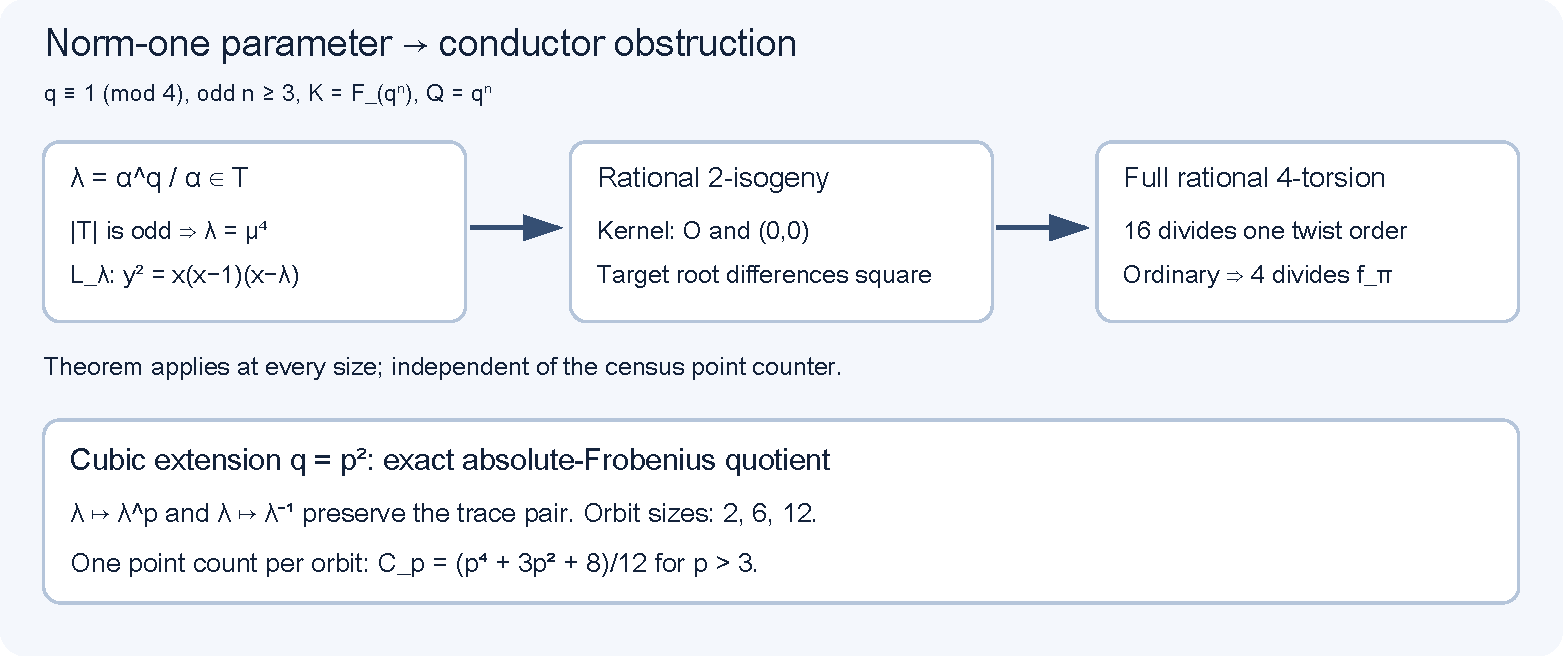
\includegraphics[width=\linewidth]{theorem_flow.pdf}
\caption{The proved implication and the orbit reduction used in the
larger-prime continuation. The census labels test the remaining
class-existence question.}
\end{figure}

\section{An exact absolute-Frobenius orbit count}
\begin{lemma}[Parameters and twist signs]\label{lem:parameters}
For $K=\F_{p^6}$ and $k=\F_{p^2}$, the map
$\alpha\mapsto\alpha^{p^2-1}$ induces a bijection
\[
 K^\times/k^\times\longrightarrow T.
\]
Removing $\lambda=1$ removes precisely the base-field line.
For each remaining parameter, the two square classes of scaling by
$k^\times$ give opposite trace signs.
\end{lemma}
\begin{proof}
The kernel is $k^\times$, and the image has cardinality
$(p^6-1)/(p^2-1)=|T|$, so it is all of $T$. A nonsquare in $k$
remains a nonsquare in the cubic extension, since the exponent
$1+p^2+p^4$ is odd. Scaling $\alpha$ by it produces the quadratic
twist. Thus a census of normalized parameters and both scaling
classes has $2(p^4+p^2)$ representatives.
\end{proof}

\begin{theorem}[Absolute-Frobenius quotient]\label{thm:orbits}
For a prime $p>3$, the action on $T\setminus\{1\}$ generated by
$\lambda\mapsto\lambda^p$ and $\lambda\mapsto\lambda^{-1}$
preserves the trace pair. Its orbit counts are
\[
 \begin{array}{c|c|c}
 \text{orbit size}&\text{number of parameters}&\text{number of orbits}\\\hline
 2&2&1\\
 6&2(p^2-1)&(p^2-1)/3\\
 12&p^4-p^2&(p^4-p^2)/12.
 \end{array}
\]
Consequently the exact number of point-count calls needed for one
representative per orbit is
\begin{equation}\label{eq:orbits}
 C_p=\frac{p^4+3p^2+8}{12}.
\end{equation}
Weighting each result by its orbit size and adding its twist sign
recovers the normalized-representative census.
\end{theorem}

\begin{proof}
The absolute Frobenius bijects rational points and preserves $T$.
Inversion preserves the Legendre cardinality because $\lambda$ is a
square: with $r^2=\lambda$, the map
$(x,y)\mapsto(x/\lambda,y/(\lambda r))$ gives
$L_\lambda\simeq L_{1/\lambda}$ over $K$.
The two operations commute and give the twelve exponents
$\pm p^j$, $0\le j<6$.

Put $A=p^2+p+1$ and $B=p^2-p+1$. Then
$|T|=AB$, $\gcd(A,B)=1$, $p^3\equiv1\pmod A$, and
$p^3\equiv-1\pmod B$. The subgroups $T_A,T_B$ have trivial
intersection. Their nonidentity union has
$A+B-2=2p^2$ elements.

The fixed-point equation for a transformation is
$\lambda^{\pm p^j-1}=1$. The identities
\[
 \gcd(AB,p^3-1)=A,\quad \gcd(AB,p^3+1)=B,
 \quad\gcd(AB,p^2-1)=3,\quad\gcd(AB,p^2+1)=1
\]
and $\gcd(AB,p\pm1)\mid3$ classify all stabilizers;
$p^6\equiv1\pmod{AB}$ reduces $j=4,5$ to $j=2,1$.
The two primitive cube roots form one orbit of size $2$.
The other $2p^2-2$ elements in $T_A\cup T_B$ have orbit size $6$.
All remaining $p^4-p^2$ elements have trivial stabilizer and orbit
size $12$. Summing the orbit counts gives~\eqref{eq:orbits}.
Lemma~\ref{lem:parameters} supplies both scaling classes and their
trace signs.
\end{proof}

\begin{center}
\begin{tabular}{rrrr}
\toprule
$p$&Normalized representatives&Six-element quotient&$C_p$\\
\midrule
13&57,460&4,789&2,423\\
37&3,751,060&312,589&156,523\\
47&9,763,780&813,649&407,193\\
53&15,786,580&1,315,549&658,243\\
59&24,241,684&2,020,141&1,010,651\\
61&27,699,124&2,308,261&1,154,751\\
199&3,136,557,604&261,379,801&130,696,501\\
\bottomrule
\end{tabular}
\end{center}
These are exact counts of parameters and point-count calls. Execution
times depend on the field kernel, the point counter, and host conditions.

\section{Evidence and the next class-existence test}
The original rational-isogeny factorization and cleared equation have
native identity records
\begin{center}
\texttt{IDC1h8ae7209125dfe0a2}\quad\texttt{IDC1he02ab9a5cf019a56}.
\end{center}
Separate exact polynomial expansion is performed in PARI/GP.
The additional halving and orbit arithmetic have records
\begin{center}
\texttt{IDC1hf8aba4800a6ceb5c}\quad\texttt{IDC1h1bc37ec40bcb8619}.
\end{center}
The generalized PARI controls passed $1{,}100$ norm-one cases and
all $476$ ordinary Hasse traces tested for the conductor equivalence.
The companion validation receipt records their frozen sources and the
larger-prime census status. The proofs above do not
depend on randomized point-count assignments.

The exact $p=7$ census counts every field element for each of the $213$
absolute orbits and agrees, including all weights, with an independent
complete PARI census. It finds $126$ weak ordinary rows among $294$,
with $20$ zero rows among the $146$ ordinary rows of depth at least two.
In particular the ordinary class $t=610$ has
\[
 Q=117{,}649,\qquad t^2-4Q=-98{,}496=72^2(-19),
 \qquad v_2(f_\pi)=3,
\]
and has no norm-one weak representative. The independent existence
check realizes this trace with three rational $2$-torsion roots; the
quadratic twist gives $t=-610$. Together with the exhaustive norm-one
enumeration, this supplies a finite, certified counterexample to
sufficiency of the depth condition for the cubic weak family.

The completed diagnostic censuses at $p=37$, $41$, $43$, $47$, and $53$
contain, respectively, 290, 396, 376, 424, and 494 ordinary zero-witness
rows at conductor depth at least two. Those rows remain labels from the
retained point counter.

The $p=53$ run has $72{,}540$ weak ordinary rows among $146{,}068$;
all $5{,}000$ independent PARI controls are in its positive set.

The next existence test is to certify those labels and test invariants
of the order containing $(\pi-1)/4$, while extending the frozen
protocol toward $p=199$. A class criterion needs a sufficient argument
for the norm-one parameter condition as well as the conductor obstruction.

\begingroup\sloppy
\begin{thebibliography}{9}
\bibitem{auertop} R. Auer and J. Top, \emph{Legendre elliptic curves
over finite fields}, 2001, Lemma 2.1 and Proposition 2.1.
\url{https://arxiv.org/abs/math/0106273}.
\bibitem{jv} A. Joux and V. Vitse, \emph{Cover and Decomposition Index
Calculus on Elliptic Curves Made Practical}, EUROCRYPT 2012.
\url{https://eprint.iacr.org/2011/020}.
\bibitem{pari} The PARI Group, \emph{PARI/GP function reference:
elliptic curves}, entries \texttt{ellcard} and \texttt{ellgroup}.
\url{https://pari.math.u-bordeaux.fr/dochtml/html/Elliptic_curves.html}.
\end{thebibliography}
\endgroup
\end{document}
